\documentclass[book,14pt,oneside,openany]{memoir}
\usepackage[utf8x]{inputenc}
\usepackage[bulgarian]{babel}
\usepackage{url}
\usepackage{lipsum}
% Според изискванията на ИИКТ-БАН не бива да има номерация на страниците в ръкописа.
\usepackage{nopageno}
\usepackage{shorttoc}
\usepackage{graphicx}
\usepackage{imakeidx}
% Добавя възможност за сензитивни хипер-връзки в самия документ.
% \usepackage{hyperref}

% Заглавие на книгата.
\title{Научни изчисления с Java и Android}

% Имена на авторите.
\author{Тодор Балабанов, Илиян Занкински, Петър Томов}

% Автоматично създаване на азбучен указател.
\makeindex[columns=1, title=Азбучен указател, intoc]

\begin{document}

\maketitle

% Заглавната страница не е с оформлението на останалата част от документа (няма номерация).
\thispagestyle{empty}

% Тук стои таблицата със съдържанието, което се генерира от названието на главите.
\newpage
\shorttoc{Теми}{0}

% Тук стои таблицата със съдържанието, което се генерира от названието на главите и названието на секциите в тях.
\newpage
\tableofcontents

% По този начин номерацията на подточките е с арабски цифри.
\renewcommand\thesection{\thechapter.\arabic{section}}
\renewcommand\thesubsection{\thesection.\arabic{subsection}}

\newpage
\addcontentsline{toc}{chapter}{Предговор}
\chapter*{Предговор}

Това учебно помагало е предназначено за ученици и студенти, които биха искали да се запознаят с възможностите за реализиране на \index{изчисления в разпределена среда} с използването на програмния език Java и мобилната платформа Android.

В съвременното ни ежедневие ние все по-често сме заобиколени от мобилни изчислителни устройства. Най-често това са мобилни телефони, таблети, часовници или други форми на wearables (миниатюрна електроника под формата на модни аксесоари или части от дрехи). До преди десетилетие този вид мобилни устройства бяха рядкост, а изчислителните им възможности бяха изключително ограничени. Тези два факта не позволяваха мобилните устройства да бъдат използвани за нещо повече освен основния принцип на употреба за който са създадени. С развитието на микроелектрониката и миниатюризацията на компонентите съставящи мобилните устройства техните възможности значително нараснаха за последното десетилетие. Това позволява върху този вид устройства да се извършват и допълнителни задачи, които не са били предвидени при първоначалното им проектиране. Паралелно с развитието на мобилните технологии бурен подем претърпяха и възможностите за мобилна комуникация като GSM, 3G, 4G, Wi-Fi, Bluetooth, NFC и други. Комбинацията между относително мощни мобилни изчислителни устройства и добре развита комуникационна среда открива безгранични възможности за приложение на мобилните устройства при извършването на допълнителни изчисления, в разпределена среда. 

В настоящето учебно помагало ще запознаем читателите с интересните възможности, които предлагат съвременните Android \index{мобилни устройства}, за постигането на резултати в научни изчислителни задачи, разпределяйки изчисленията върху физически отдалечени едно от друго устройства. 

\newpage
\chapter{Научни изчисления}

Още в зората на съвременната изчислителна техника най-съществените пресмятания са били с научна насоченост и военно дело. Този факт не се е променил значително за последните десетилетия. Дори в наши дни най-сериозните изчислителни ресурси са насочени в областта на науката. Това дава основание да обърнем значително внимание на начините по които можем да изпълняваме научни изчисления дори и върху изчислителни устройства, чието основно предназначение не е с научна цел. 

\section{Последователно програмиране}

При \index{последователното програмиране} всяка изчислителна инструкция следва всички предходни. В зората на изчислителната техника пресмятанията са извършвани по този начин. Дори в наши дни значителна част от алгоритмите се изпълняват само последователно, тъй като входните данни за всяка инструкция зависят от изходните данни на предходните инструкции. Последователните алгоритми не подлежат на декомпозиране и поради тази причина са неприложими за паралелни пресмятания. 

\begin{figure}[h!]
  \centering
  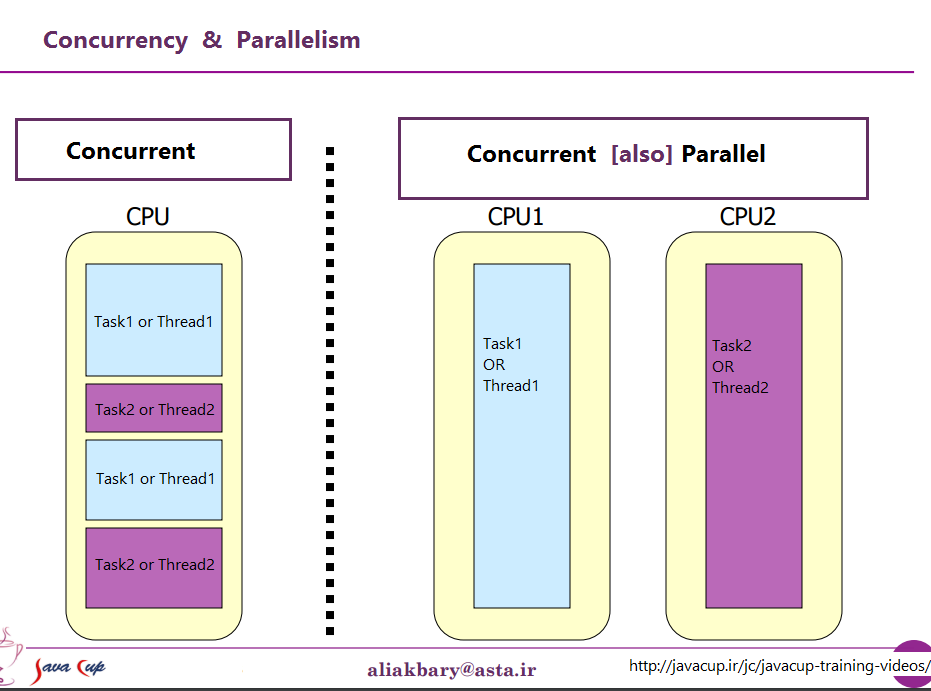
\includegraphics[width=1.0\linewidth]{./images/pic0001.png}
  \caption{Сравнение между последователни пресмятания и паралелни пресмятания.}
\label{fig:pic0001}
\end{figure}

\section{Паралелно програмиране}

При паралелното програмиране основно се говоир за две разновидности - \index{конкурентни пресмятания} и \index{паралелни пресмятания}. Конкурентните пресмятания са в среда където група от задачи могат да се пресметнат едновременно, без да има значение от реда на пресмятане. В същото време, паралелните пресмятания се отнасят за едновременно пресмятане на отделни задачи, върху отделни процесори. В този контекст всички паралелни пресмятания са конкурентни пресмятания, но не и обратното (Фиг. \ref{fig:pic0001}). 

\begin{figure}[h!]
  \centering
  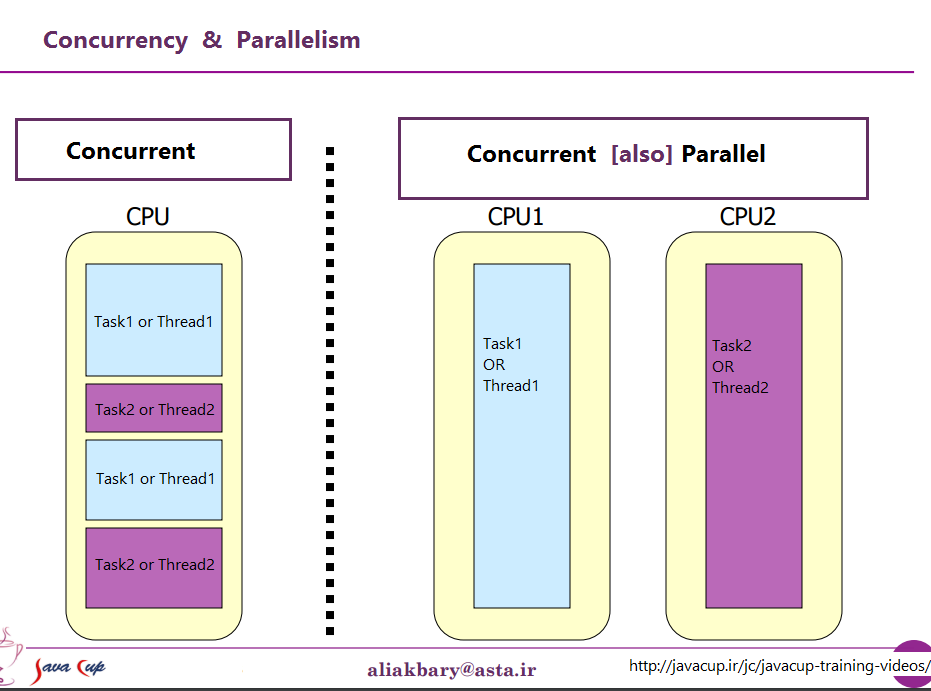
\includegraphics[width=1.0\linewidth]{./images/pic0002.png}
  \caption{Сравнение между конкуретни пресмятания и паралелни пресмятания.}
\label{fig:pic0002}
\end{figure}

\section{Супер компютри и грид изчисления}

Когато паралелните алгоритми се изпълняват на изчислителни машини с множество процесори и/или множество ядра на процесорите, този вид изчисления се определят като супер компютърни (supercomputing). Същественото при този вид пресмятания е, че се използва много бърз вътрешна шина (понякога оптична) и споделена оперативна памет. За разлика от \index{супер компютрите} \index{грид изчисленията} се осъществяват на множество машини, свързани в обща мрежа, но работещи автономно, без да споделят обща памет. При грид системите отделните изчислителни машини могат да са териториално отдалечени една от друга. Съществено е да се отбележи, че и при супер компютрите собственикът на системата има пълен контрол над нея. Това може малко да се различава за грид системите, ако към грида са включени компютри под чужд контрол. 

\section{Изчисления в разпределена среда}

Преходът от грид системите към системи за \index{изчисления в разпределена среда} се състои в това, че изчислителните машини в разпределената среда са абсолютно автономни. Тези машини не споделят общи ресурси, като процесор или оперативна памет. Много характерно е в разпределената среда контролът над изчислителните машини да не е от страната на организиращия изчисленията. Това води до два основни проблема - ненадеждна (често и твърде бавна) комуникация, липса на гаранция за коректност на пресмятанията (манипулации от страна на притежаващия изчислителните ресурси). Също така, при грид системите често се наблюдава хомогенност на изчислителните ресурси по отношение на хардуерни конфигурации и операционна система, докато в разпределената среда изчислителните машини са основно хетерогенни, което може да води до големи разлики в хардуера и операционните системи. 

\section{Дарена изчислителна мощност}

За решаването на някои по-мащабни научни проблеми изчислителната мощност и/или финансовите ресурси често са недостатъчни. В такива ситуации не малко научни институции прибягват до така наречените \index{дарени изчислителни ресурси} в \index{разпределена среда}. Един от най-изчерпателните списъци с проекти от този вид може да бъде открит в уеб сайта Distributed Computing Info \cite{dcinfo}. Съществено е да се отбележи, че не всеки изчислителен проблем е подходящ за решение в \index{разпределена среда} с дарена изчислителна мощ. На първо място проблемът трябва да подлежи на декомпозиране, така че отделни части от него да се пресмятат едновременно. Второто важно нещо е да не е от съществено значение в кой момент от времето и в какъв ред ще бъдат получени пресметнатите резултати. И третото съществено нещо е да е наличен механизъм за проверка на достоверността от пресмятанията, тъй като изчисленията се извършват на машини с различна хардуерна конфигурация и различни операционни системи, а освен това са възможни манипулации от страна на хората притежаващи тези машини. Най-известният проект за дарена изчислителна мощ е SETI@home \cite{shuch}, като неговата цел е да търси сигнали от космоса, които да са създадени от интелигентни форми наживот.

Когато изчисленията се извършват на мобилни устройства, то разпределената среда се превръща в \index{мобилна среда за разпределени изчисления}. В останалата част от това учебно помагало ще бъде представено точно изграждането на система за извършване на разпределени изчисления върху мобилни устройства. 
\newpage
\chapter{Евристични алгоритми}

Евристичните алгоритми са подход за решаване на изчислителни проблеми, основаващи се на опита и интуицията. Този вид алгоритми не гарантират оптимално решение за поставената задача. Евристичните алгоритми намират широко приложение при задачи, които трудно се поддават на точни числени методи или аналитични решения. Макар и да не могат да предложат оптимално решение, \index{евристичните алгоритми} често водят до достатъчно приемливи в практиката, близки до оптималното решения. Благодарение на своята не детерминистична природа, \index{евристичните алгоритми} са изключително подходящи за реализация в супер компютърни изчисления. Две изключително популярни \index{евристики} са \index{изкуствените неверонни мрежи} и \index{генетичните алгоритми}. Те са обект на особена популярност през последните две десетилетия и това дава основание да бъдат заложени в основното изложение на настоящото учебно помагало. Сами по себе си евристиките са безполезни, ако не бъдат приложени върху достатъчно сложна изчислителна задача. Точно такава сложност предлагат задачите за прогнозиране. Прогнозирането е залегнало в множество дейности от човешкото ежедневие, като започнем от средните дневни температури и стигнем до потреблението на определени стоки и услуги. Под една или друга форма почти всяка човешка дейност бива остойностена в термините на финансовите ресурси. Този факт дава основание да бъдат разгледани точно прогнози за промяната в цените на различни финансови инструменти. Отчитането на промяната в цената, на определени интервали (равни или неравни), води до представяне на информацията във \index{времеви ред}. При \index{времевите редове} по абсцисната ос се означава времето, а по ординатната ос стойността на измерваната величина (в конкретния случай цената).

\section{Финансови времеви редове}

\begin{figure}[h!]
  \centering
  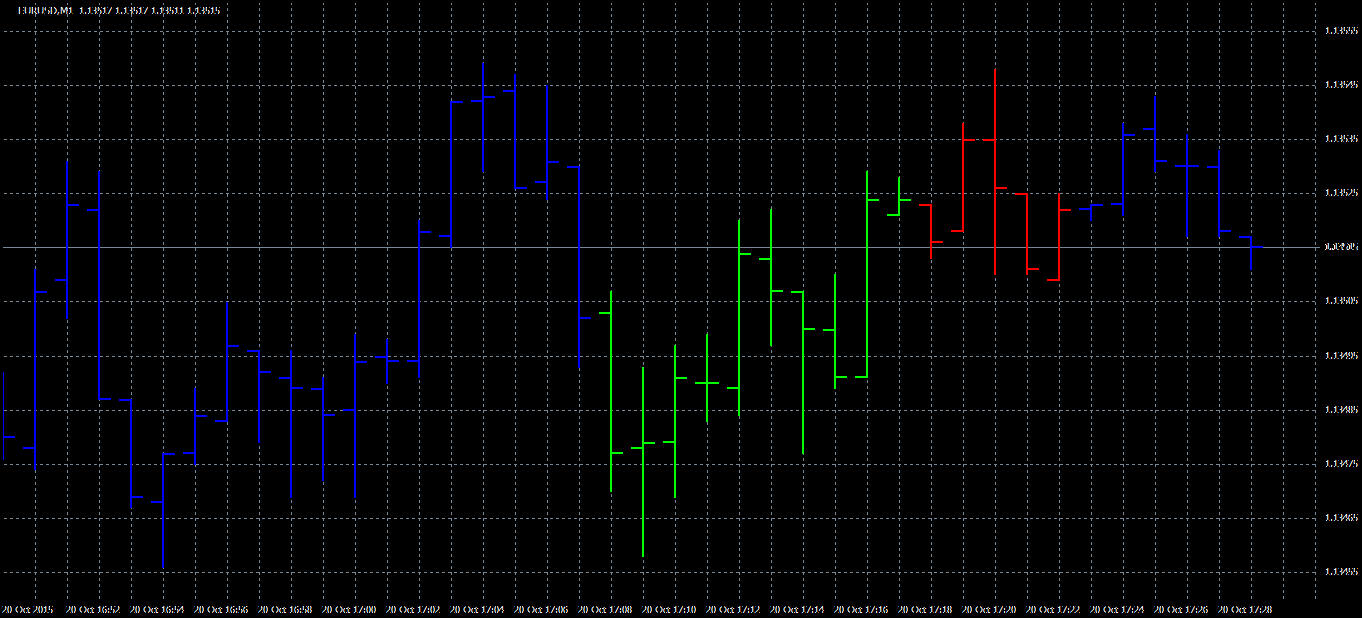
\includegraphics[width=1.0\linewidth]{./images/pic0003.png}
  \caption{Отношението евро/долар в рамките на един час.}
\label{fig:pic0003}
\end{figure}

\section{Изкуствени невронни мрежи}

\begin{figure}[h!]
  \centering
  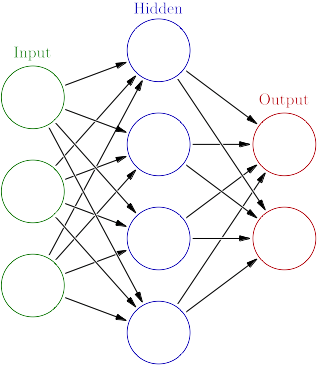
\includegraphics[height=0.5\pdfpageheight]{./images/pic0004.png}
  \caption{Трислойна изкуствена невронна мрежа.}
\label{fig:pic0004}
\end{figure}

\section{Генетични алгоритми}

\begin{figure}[h!]
  \centering
  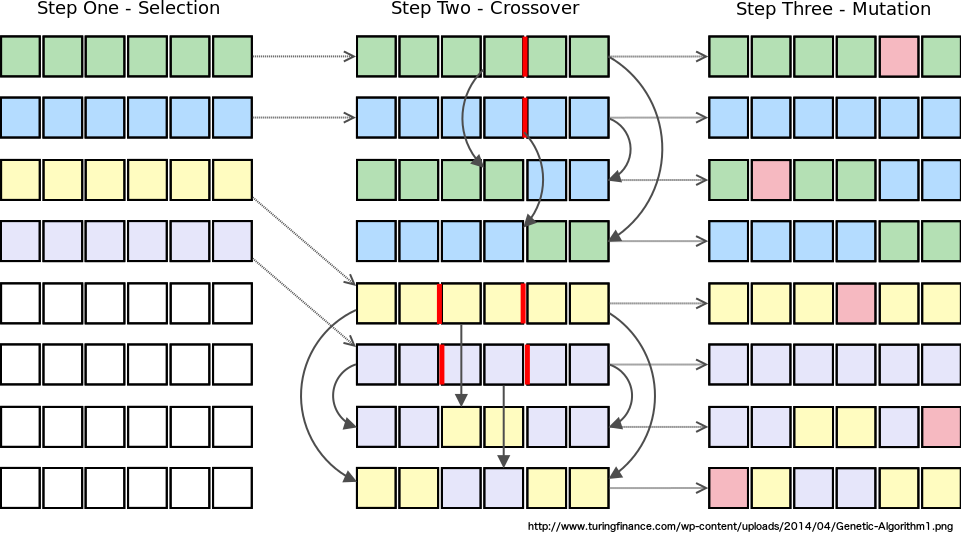
\includegraphics[width=1.0\linewidth]{./images/pic0005.png}
  \caption{Трите основни операции в генетичните алгоритми.}
\label{fig:pic0005}
\end{figure}

\section{Прогнозиране в разпределена среда}

Гъвкавите възможности на \index{изкуствените невронни мрежи} да изграждат функционална зависимост между входни и изходни данни ги прави идеален кандидат за прогнозираща система. Ако се приеме, че измерените стойности във времевия ред са точки в двуизмерно пространство, то задачата за прогнозиране може да се представи като задача за прекарване на крива през N точки (curve fitting). Ако образно се оприличи изкуствената невронна мрежа на полином, то теглата й биха представлявали коефициенти в полинома. Стойностите които \index{изкуствената невронна мрежа} генерира на изхода си за бъдещи моменти от времето представляват своеобразна \index{екстраполация} според апроксимираната крива. Тъй като класическите многослойни невронни мрежи работят с входни сигнали между 0.0 и 1.0 или -1.0 и +1.0, то информацията от времевия ред трябва да бъде мащабирана в съответния работен интервал на мрежата. Стойностите на времевия ред условно се разделят на минали (зелените Фиг. \ref{fig:pic0003}) и бъдещи (червените Фиг. \ref{fig:pic0003}). Изходната (прогнозна) информация на изкуствената невронна мрежа след това се мащабира обратно към оригиналните интервали на времевия ред.

\begin{figure}[h!]
  \centering
  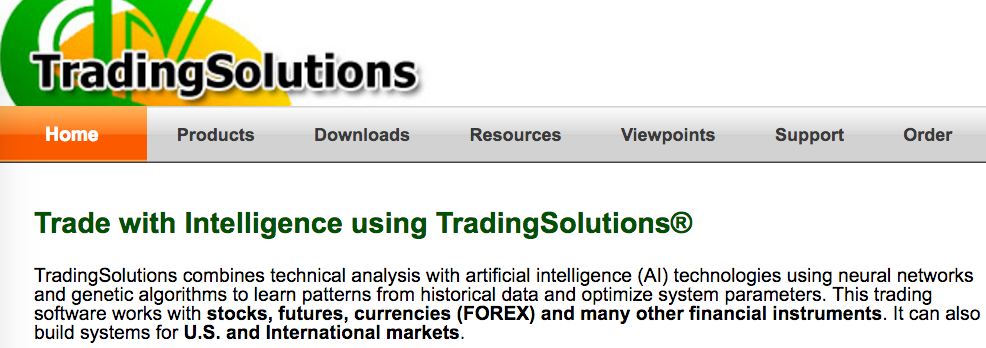
\includegraphics[width=1.0\linewidth]{./images/pic0006.png}
  \caption{Продуктовата линия TradingSolutions използваща изкуствени невронни мрежи и генетични алгоритми за прогнозиране на Forex финансови инструменти.}
\label{fig:pic0006}
\end{figure}

От чисто практическа гледна точка, използването на изкуствени невронни мрежи и генетични алгоритми се е доказало като удачен подхода за прогнозиране на финансови инструменти, което ясно се вижда в продуктовата линия на TradingSolutions (Фиг. \ref{fig:pic0006}). Почти петнадесет години продуктовата линия на TradingSolutions доставяше \index{системи за подпомагане вземането на решения}. По настояще тази продуктова линия е придобита от компанията nDimensional, Inc.

\begin{figure}[h!]
  \centering
  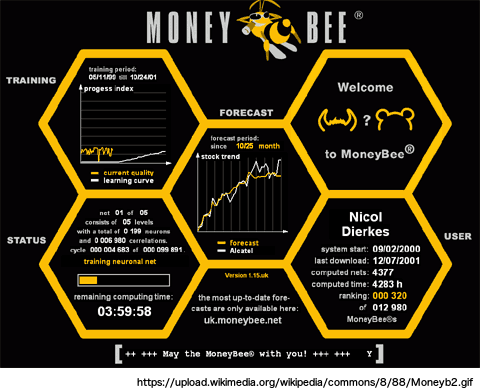
\includegraphics[height=0.4\pdfpageheight]{./images/pic0007.png}
  \caption{Системата MoneyBee за финансово прогнозиране в разпределена среда.}
\label{fig:pic0007}
\end{figure}

Възможността да се прогнозират цените на финансови инструменти винаги е привличала не само индустрията, но и научните среди. Едно от най-забележителните постижения в тази насока е проектът MoneyBee (Фиг. \ref{fig:pic0007}). Макар и вече да не съществува, този проект предлагаше възможност за изчисляване на прогнози с помощта на \index{дарена изчислителна мощност} в \index{разпределена среда} \cite{bohn}. Същинските прогнози се пресмятаха, с помощта на изкуствени неверонни мрежи, върху изчислителните машини на потребителите в периоди когато натоварването на машините е ниско и се активира програмата за защита на монитора (screensaver). Преди масовото навлизане на мобилните устройства честа практика при проектите за дарена изчислителна мощност, с цел пресмятане в разпределена среда, основен подход бе извършване на пресмятанията в специално създадена за целта програма за предпазване на монитора. След навлизането на катодно лъчевите тръби при настолните компютри се появява ефект от увреждане на монитора, ако върху него продължително се визуализира статична картина. Решаването на този проблем се оказва най-удачно с помощта на операционната система, която да установи период в който потребителя не използва изчислителната машина и да активира софтуерна програма за предпазване на монитора. Развитието на мониторите с течни кристали постепенно изведе от употреба мониторите с катодно-лъчеви тръби и използването на програми за предпазване на монитора изгуби своето първоначално предназначение. Въпреки това този вид софтуерни решения останаха в употреба и основно служат за повишаване на информационната сигурност, като не само дават естетическа визуализация, но и привеждат работната сесия на потребителя в заключено състояние, което възпрепятства използването на компютърната система от неауторизирани потребители. Наличието на изчислителни ресурси, които са налични, но неефективно използвани дава основание на множество учени да разработят системи за отдалечено пресмятане в \index{разпределена среда}, точно под формата на програми за предпазване на монитора, които да се възползват от дарените потребителски, изчислителни ресурси. 

\section{Фонови пресмятания върху мобилни устройства}

Съществува концептуална разлика в начина по който потребителите използват настолните си компютри и мобилните устройства. На първо място, настолният компютър бива пускан и спиран според нуждите на потребителя, докато най-често мобилните устройства са в непрекъснат режим на употреба. Това води до основната разлика, че мобилните устройства не изпадат в режим на занижена употреба, но също така имат режими за употреба при изключителна важност (примерно телефонно обаждане с висок приоритет). Втората фундаментална разлика се състои във факта, че основен похват за пестене на електрическа енергия, доставяна предимно от батерии при мобилните устройства, е динамичното изгасяне на екрана. Тази стратегия за пестене на енергия кардинално отменя концепцията за програма предпазваща монитора. За да се реализира ефективно система за разпределени пресмятания върху мобилни устройства е много по-удачно да се използва технологията за активен десктоп, отколкото да се залага да идеята за програма предпазваща монитора. Точно тази идея е развита в настоящото учебно помагало. 

\newpage
\addcontentsline{toc}{chapter}{Заключение}
\chapter*{Заключение}

Основна цел на настоящото учебно помагало бе представянето на възможностите, които съвременните Android мобилни устройства могат да предложат за извършване на научни изчисления в разпределена среда. Без да претендира за изчерпателност изложеният материал има за цел да провокира творческото мислене у читателя и да го вдъхнови за създаването на собствени авторски проекти с разгледаните технологии и засегнатите научни области.  

Авторите са благодарни на своите читатели за отделеното време и внимание, като горещо насърчават подаването на обратна връзка и споделянето на интересни мисли, идеи или предложения, на посочените за връзка контакти.

% Списък с използвана литература и източници на информация.
\newpage
\begin{thebibliography}{99}

\bibitem{dcinfo} Distributed Computing Info , \\\texttt{http://www.distributedcomputing.info/}

\bibitem{shuch} Paul Shuch, H. \textit{Searching for Extraterrestrial Intelligence}. Springer-Verlag Berlin Heidelberg, 2011.

\bibitem{bohn} Bohn, A., Guting, T., Mansmann, T. \textit{MoneyBee: A new product to predict stock market developments using artificial intelligence and increased calculation capacitiy} German. et al. Wirtschaftsinf, vol. 45/3, 325--333, 2003.

\end{thebibliography}

% Азбучен указател на използваните термини.
\newpage
\printindex

\end{document}